\section{$2 \times 2 \times k$ Table}
\subsection{Setup}
The data consist of $k$ strata, $i = 1, 2, \cdots, k$. Within each stratum, we have a $2 \times 2$ table.
\begin{figure}[H]
	\centering
	
\includegraphics[width=0.7\linewidth]{fig/screenshot004}
	\caption{One of the Stratum}
	\label{fig:screenshot005}
\end{figure}
The two rows of the $2 \times 2$ table in the $i$-th stratum are viewed
as data from two independent binomial distributions.

\begin{figure}[H]
	\centering
	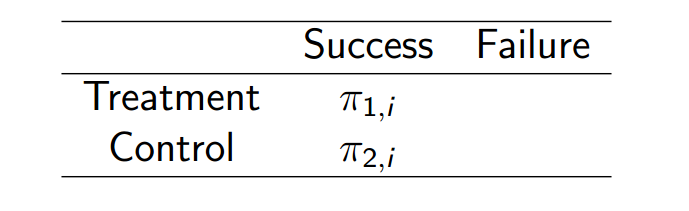
\includegraphics[width=0.5\linewidth]{fig/screenshot006}
	\caption{Probabilities in One of the Stratum}
	\label{fig:screenshot006}
\end{figure}

\subsection{Hypothesis Test}
Null hypothesis is that within each straum, the success probabilities are equal.
\[H_0: \pi_{1, i} = \pi_{2, i}, i = 1, \cdots, k.\]

Let $\theta$ denote the odds ratio for the $i$-th table.
\[\theta_i = \frac{\pi_{1, i}/ (1 - \pi_{1, i})}{\pi_{2,i}/ (1 - \pi_{2, i})}\]

Use odds ratio to represent the null hypothesis.
\[H_0: \theta_1 = \theta_2 = \cdots = \theta_k = 1\]

Note that we are testing that there is a common odds ratio and it is equal
to 1.
Moreover, $H_0$ allows for the common success probabilities to differ from
stratum to stratum.

Note that the alternative hypothesis must be consistent across the stratum. By consistent, I mean it is either
\[H_1: \pi_{1,i} \ge \pi_{2,i} \text{ for all } i = 1, \cdots, k \text{ with at least one inqeuality.}\]
or
\[H_1: \pi_{1,i} \le \pi_{2,i} \text{ for all } i = 1, \cdots, k \text{ with at least one inqeuality.}\]